\documentclass{beamer}
\usepackage[utf8]{inputenc}
\usetheme{Madrid}
\usecolortheme{default}
\usepackage{amsmath,amssymb,amsfonts,amsthm}
\usepackage{txfonts}
\usepackage{tkz-euclide}
\usepackage{listings}
\usepackage[T1]{fontenc}
\usepackage{adjustbox}
\usepackage{array}
\usepackage{tabularx}
\usepackage{gvv}
\usepackage{lmodern}
\usepackage{circuitikz}
\usepackage{tikz}
\usepackage{graphicx}
\setbeamertemplate{page number in head/foot}[totalframenumber]

\title{7.2.5}
\author{AI25BTECH11014 - Gooty Suhas}
\begin{document}
\frame{\titlepage}

\begin{frame}{Problem}
Check whether the point \( \vec{P} = \myvec{-2 \\ 4} \) lies on a circle of radius 6 centered at  
\( \vec{C} = \myvec{3 \\ 5} \).
\end{frame}

\begin{frame}{Matrix Form}
The general equation of a circle with center \( \vec{C} \) and radius \( r \) is:
\[
\|\vec{x} - \vec{C}\|^2 = r^2
\]
Substituting \( \vec{C} = \myvec{3 \\ 5} \), \( r = 6 \):
\[
\|\vec{x} - \myvec{3 \\ 5}\|^2 = 36
\]
Expanding the norm:
\[
(\vec{x} - \myvec{3 \\ 5})^T (\vec{x} - \myvec{3 \\ 5}) = 36
\]
\end{frame}






\begin{frame}{Substitution}
Let \( \vec{x} = \vec{P} = \myvec{-2 \\ 4} \). Then:
\[
\vec{x} - \vec{C} = \myvec{-2 \\ 4} - \myvec{3 \\ 5} = \myvec{-5 \\ -1}
\]
Now compute the squared norm:
\[
\|\vec{x} - \vec{C}\|^2 = \myvec{-5 \\ -1}^T \myvec{-5 \\ -1}
= (-5)^2 + (-1)^2 = 25 + 1 = 26
\]
So the point yields:
\[
\|\vec{P} - \vec{C}\|^2 = 26
\]
\end{frame}






\begin{frame}{Comparison}
\[
\text{LHS} = 26, \quad \text{RHS} = 36
\Rightarrow 26 \ne 36
\]
\end{frame}

\begin{frame}{Conclusion}
The point \( \vec{P} = \myvec{-2 \\ 4} \) does not satisfy the equation of the circle.  
Hence,  
\[
\boxed{\vec{P} \text{ does not lie on the circle}}
\]
\end{frame}

\begin{frame}[fragile]{verify\_circle.py (Part 1)}
\begin{lstlisting}[language=Python]
from sympy import Matrix, simplify

P = Matrix([[-2], [4]])
C = Matrix([[3], [5]])
r_squared = 36

diff = P - C
distance_squared = simplify(
    diff.T * diff
)[0]
\end{lstlisting}
\end{frame}

\begin{frame}[fragile]{verify\_circle.py (Part 2)}
\begin{lstlisting}[language=Python]
print("Distance squared:",
      distance_squared)
print("Radius squared:",
      r_squared)

print("Point lies on circle:",
      distance_squared == r_squared)
\end{lstlisting}
\end{frame}

\begin{frame}[fragile]{verify\_circle.c (Part 1)}
\begin{lstlisting}[language=C]
#include <math.h>

void verify_circle(float px, float py,
                   float cx, float cy,
                   float radius,
                   float* result) {
  float dx = px - cx;
  float dy = py - cy;
\end{lstlisting}
\end{frame}

\begin{frame}[fragile]{verify\_circle.c (Part 2)}
\begin{lstlisting}[language=C]
  float dist_sq = dx*dx + dy*dy;
  float r_sq = radius * radius;

  if (fabs(dist_sq - r_sq) < 1e-6)
    *result = 1.0;
  else
    *result = 0.0;
}
\end{lstlisting}
\end{frame}

\begin{frame}[fragile]{call\_verify.py (Part 1)}
\begin{lstlisting}[language=Python]
import ctypes

lib = ctypes.CDLL('./libverify.so')

lib.verify_circle.argtypes = [
    ctypes.c_float, ctypes.c_float,
    ctypes.c_float, ctypes.c_float,
    ctypes.c_float,
    ctypes.POINTER(ctypes.c_float)
]
\end{lstlisting}
\end{frame}

\begin{frame}[fragile]{call\_verify.py (Part 2)}
\begin{lstlisting}[language=Python]
lib.verify_circle.restype = None

px, py = ctypes.c_float(-2.0), ctypes.c_float(4.0)
cx, cy = ctypes.c_float(3.0), ctypes.c_float(5.0)
radius = ctypes.c_float(6.0)
result = ctypes.c_float()

lib.verify_circle(px, py, cx, cy,
                  radius, ctypes.byref(result))
\end{lstlisting}
\end{frame}

\begin{frame}[fragile]{call\_verify.py (Part 3)}
\begin{lstlisting}[language=Python]
if result.value == 1.0:
    print("Verified: Point lies on the circle")
else:
    print("Verified: Point does NOT lie on the circle")
\end{lstlisting}
\end{frame}



\begin{frame}{Diagram}
\centering
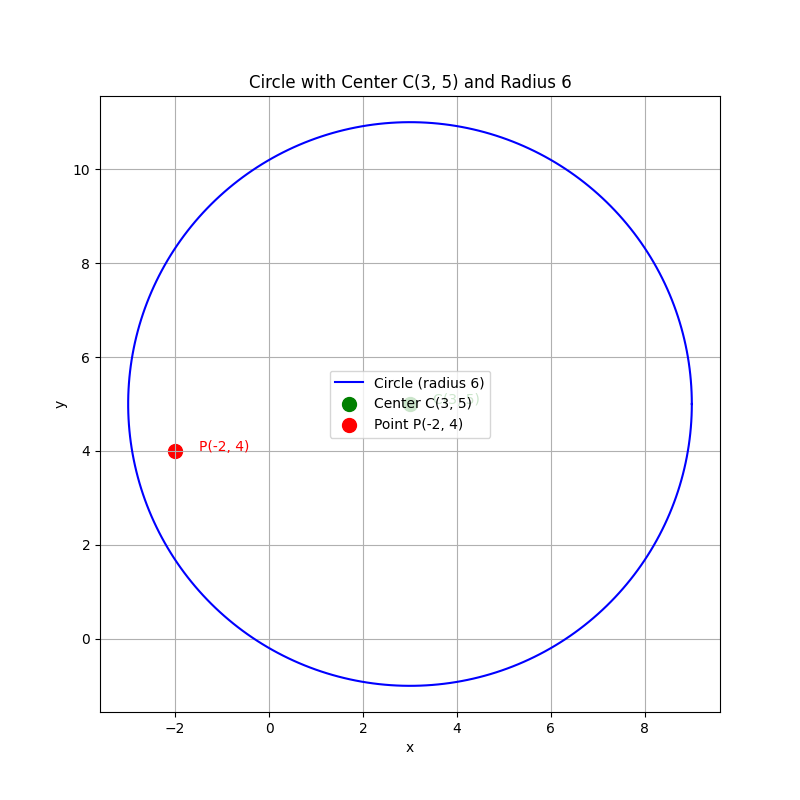
\includegraphics[width=0.7\linewidth]{Figs/Fig1.png}
\captionof{figure}{Circle and the point}
\end{frame}

\end{document}







